\documentclass[10pt,a4paper]{article}
\usepackage[a4paper,margin=1.5cm,includefoot]{geometry}
\usepackage[T1]{fontenc}
\usepackage{lmodern}
\usepackage{microtype}
\usepackage{graphicx}
\usepackage{booktabs}
\usepackage{caption}
\usepackage{hyperref}
\usepackage{xcolor}
\usepackage{enumitem}
\usepackage{fancyhdr}
\usepackage{float}
\usepackage{amsmath}
\usepackage{wrapfig}

% ---- Repository link: replace with the private GitHub repository URL before submission ----
\newcommand{\repo}{https://github.com/chairlamp/brats-3d-unet-segmentation}

\captionsetup{font=small,labelfont=bf,skip=3pt}
\setlist{nosep,leftmargin=1.2em}
\setlength{\parskip}{3pt}
\setlength{\parindent}{0pt}
\setlength{\textfloatsep}{8pt plus 2pt minus 2pt}
\setlength{\floatsep}{6pt plus 2pt minus 2pt}
\hypersetup{colorlinks=true,linkcolor=black,citecolor=black,urlcolor=blue!50!black}
\pagestyle{fancy}
\fancyhf{}
\renewcommand{\headrulewidth}{0pt}
\fancyfoot[L]{\footnotesize ENG2440 A2 \textbullet{} Aschalew Mathewos Damtew, 25011094 \textbullet{} Repository: \url{\repo}}
\fancyfoot[R]{\footnotesize \thepage}
\newcommand{\mL}{\,mL}
\newcommand{\mm}{\,mm}

\begin{document}

{\centering
{\Large\bfseries Whole-tumour segmentation in multimodal 3D MRI}\\[3pt]
{\large ENG2440 Assignment 2 \quad Aschalew Mathewos Damtew \quad 25011094}\\[3pt]
{\small Private repository (executed notebook \texttt{25011094\_ENG2440\_A2.ipynb}, \texttt{a2/} code, README, environment, AI-use declaration): \url{\repo}}\par}
\vspace{4pt}

\section{Task definition}
\textbf{Input:} one patient case, a co-registered, skull-stripped 4-channel MRI volume (FLAIR, T1w, contrast-enhanced T1 = T1gd, T2w), $240\times240\times155$ voxels at 1\mm{} isotropic spacing, as a tensor $[4,D,H,W]$. \textbf{Output:} a binary whole-tumour mask on the same grid, $[1,D,H,W]$, with $y(v)=1$ if voxel $v$ carries any tumour sub-region label (edema 1, non-enhancing tumour 2, enhancing tumour 3). \textbf{Unit of analysis:} the patient case; in MSD Task01 one case is one 4-channel volume plus one label volume, so splits, metrics and summaries are per case. A \emph{voxel} is one $1\times1\times1$\mm$^3$ sample with four intensities and one label; a \emph{slice} is the 2D plane of voxels at one index along one axis; a \emph{volume} is the full 3D grid of one acquisition. \textbf{Intended technical use:} automatic delineation of whole-tumour extent and volume (mL) for studying volumetric segmentation methods. The target is a research reference annotation, not pathology-confirmed extent; nothing here establishes clinical safety or suitability for treatment planning.

\section{Data, geometry and split}
MSD Task01 BrainTumour~\cite{antonelli2022,msd2018}, derived from BraTS 2016/2017~\cite{menze2015}: the 484 labelled cases of \texttt{imagesTr/} and \texttt{labelsTr/}. All 484 headers agree: image $240\times240\times155\times4$ float32, label $240\times240\times155$ uint8, spacing $1\times1\times1$\mm, identity affine (orientation codes RAS), image and label affines equal, label values $\{0,1,2,3\}$; channel order FLAIR, T1w, T1gd, T2w from \texttt{dataset.json}. Figure~\ref{fig:modalities} shows the four channels at one physical location (one 4D file, one affine, so voxel $(i,j,k)$ is the same point in every channel).

\begin{figure}[H]
\centering
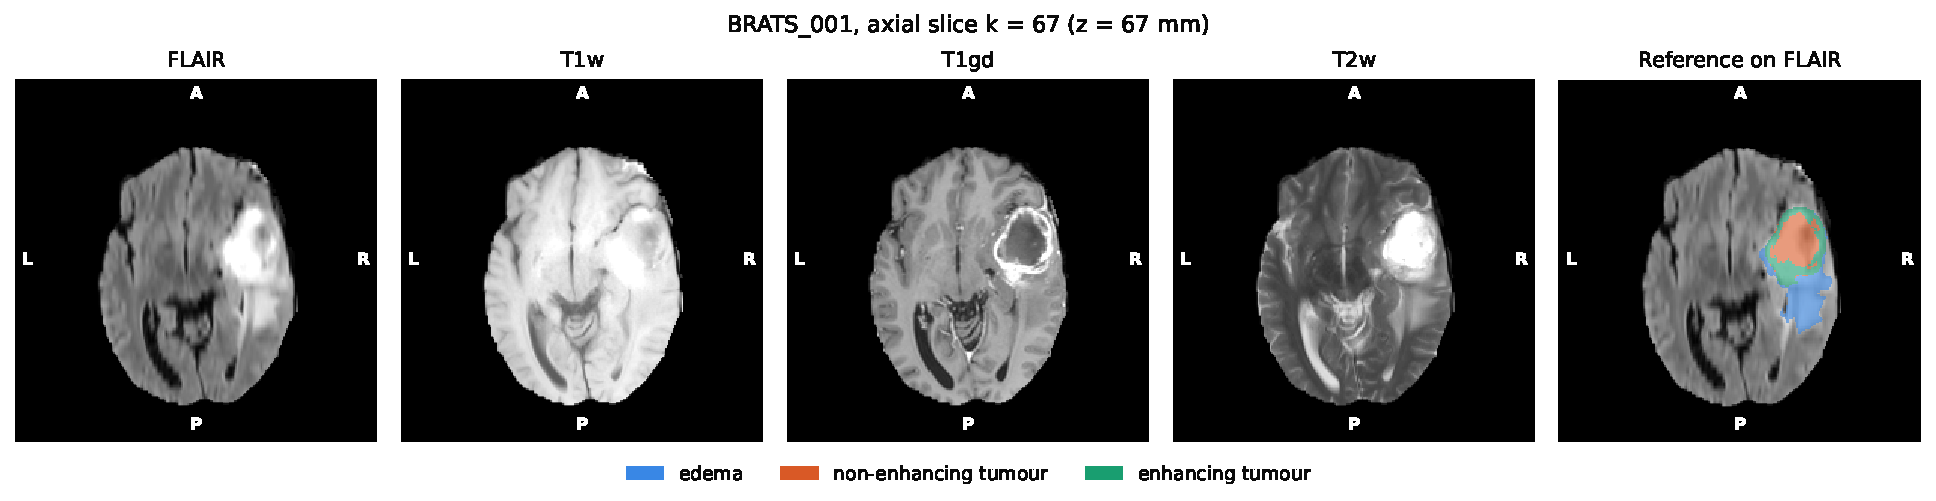
\includegraphics[width=\textwidth]{figures/fig_modalities.pdf}
\caption{BRATS\_001 (training case), axial slice through the tumour centre of mass ($z=67$\mm), all four channels and the reference sub-regions on FLAIR. Orientation letters come from the affine.}
\label{fig:modalities}
\end{figure}

\begin{wrapfigure}{r}{0.52\textwidth}
\vspace{-10pt}
\centering
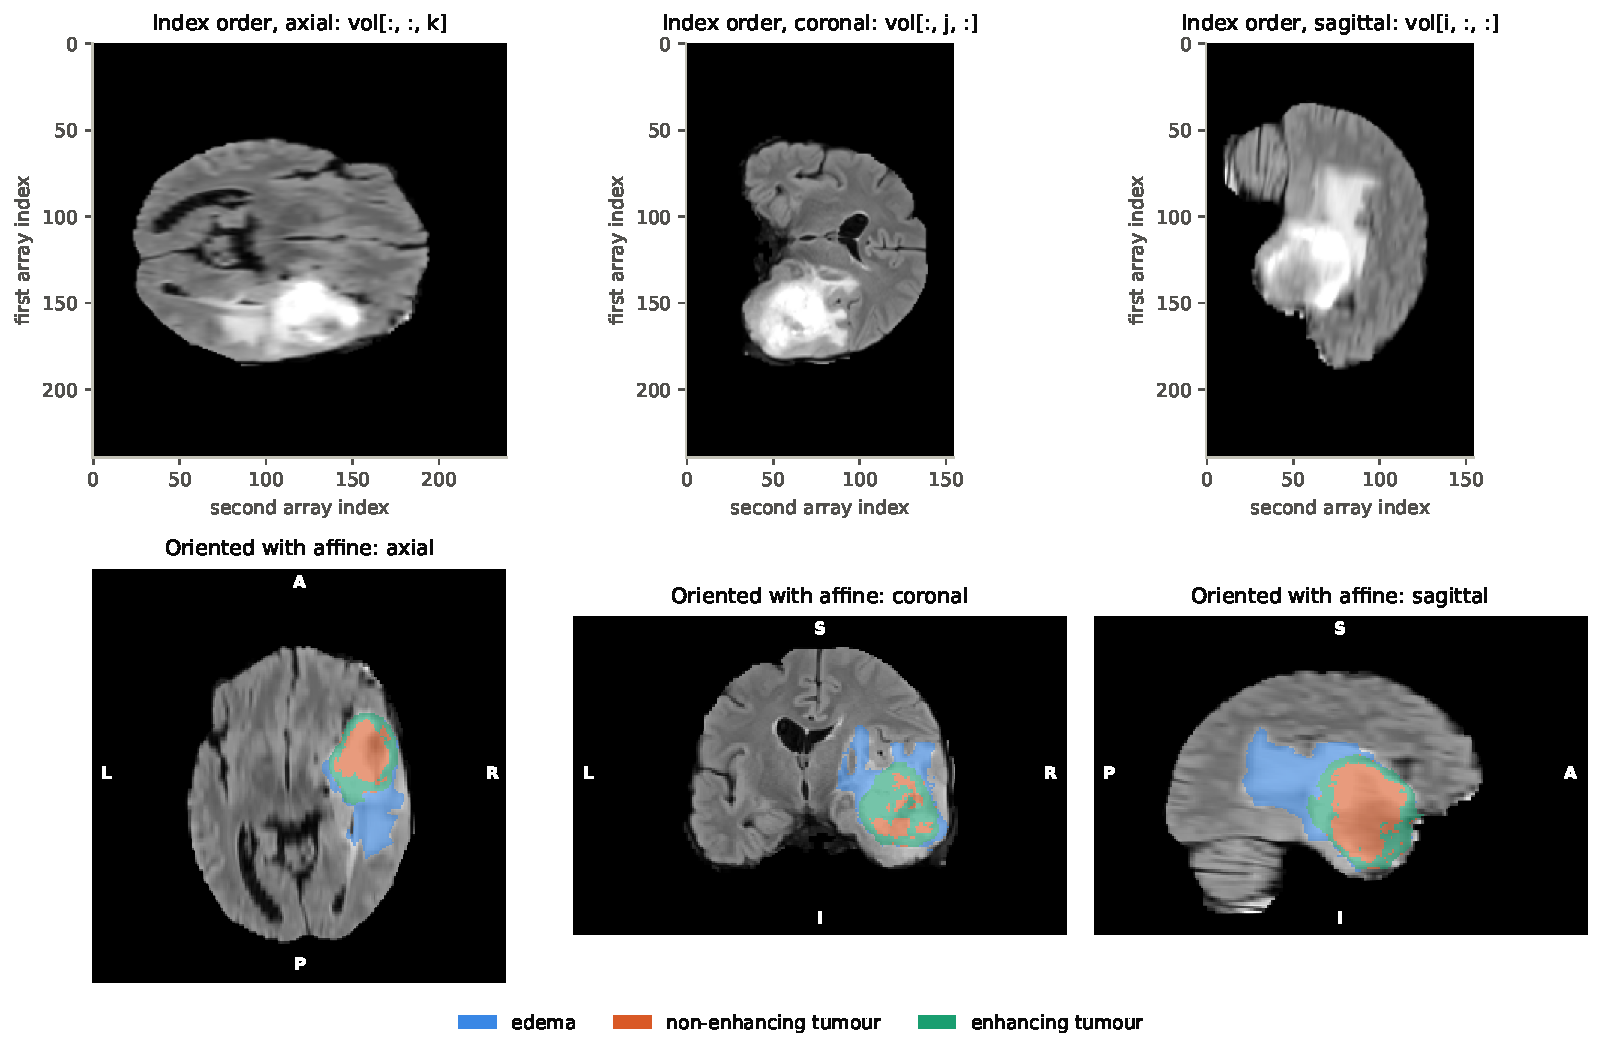
\includegraphics[width=0.52\textwidth]{figures/fig_planes.pdf}
\caption{Top: raw array in file-index order with matplotlib defaults. Bottom: the same voxels reoriented with the affine, with the reference overlaid.}
\label{fig:planes}
\vspace{-8pt}
\end{wrapfigure}
\textbf{Why file-index order is insufficient (Fig.~\ref{fig:planes}).} An array is a grid of indices; which anatomical direction each index runs along, and how far apart voxels are, is stored only in the affine. Displayed in index order, every plane appears rotated by $90^\circ$ and the sagittal head lies on its side; nothing in the array says which side is anterior, superior or left. Reading the affine (here: $+i$ towards patient right, $+j$ anterior, $+k$ superior, 1\mm{} apart) gives the correct layout, and the same code handles files stored in LPS or oblique orientations, where a hard-coded transpose would silently mirror the anatomy. Spacing must also set the display aspect and convert counts to mm and mL, and only world coordinates (mm) make positions comparable across scans. The anatomy confirms the header's anterior and superior directions (the cerebellum lies at low $j$ and $k$); left--right cannot be verified from a nearly symmetric brain, so no laterality claims are made.

\textbf{Split.} \texttt{assignment2\_split.csv} is used unchanged; patches are drawn on the fly from training cases only. The brief's setup check passes; every listed file exists, case IDs are unique and disjoint, each file name matches its case ID, and the split covers exactly the 484 archive cases. Test labels are read only for the cache, this table and the duplicate check below; no decision uses them before Section~\ref{sec:test}.

\begin{table}[H]
\centering\small
\caption{Cases and reference whole-tumour volume (mL) per split.}
\label{tab:split}
\begin{tabular}{@{}lrrrrrr@{}}\toprule
Split & Cases & Mean & SD & Median & IQR & Range \\\midrule
Train & 338 & 103.0 & 57.0 & 95.5 & 60.0--143.9 & 8.5--265.3 \\
Validation & 73 & 100.8 & 63.0 & 91.6 & 51.9--148.1 & 7.3--266.9 \\
Test & 73 & 107.4 & 66.3 & 89.1 & 54.4--157.7 & 10.1--318.3 \\\bottomrule
\end{tabular}
\end{table}

\textbf{Hidden overlap: near-duplicate scans.} Disjoint case IDs do not guarantee disjoint scans. Comparing coarse, intensity-normalised FLAIR/T2w fingerprints of all 117{,}000 case pairs found \textbf{116 pairs with correlation $\geq 0.9998$}, separated by a clear gap from all other pairs (maximum 0.962): IDs 1--274 and 275--479 contain the same images, so the 484 cases hold only 368 distinct scans. Only 6 of the 116 pairs have identical label files; the two annotations of the same images agree at a mean whole-tumour Dice of 0.922 (min 0.649). Across splits, 23 pairs join train and test and 6 join validation and test, so \textbf{29 of the 73 test cases} (and 26 of the 73 validation cases) have a twin scan used in training or selection. The split is kept as required; Section~\ref{sec:test} reports the effect.

\section{Safe preprocessing}
\textbf{Geometry and target grid.} Every case is already on one common grid ($240\times240\times155$, 1\mm{} isotropic, RAS), which is the target grid; no resampling was needed (the pipeline would resample with linear interpolation for MRI and nearest neighbour for labels, and records that it never did). \textbf{Interpolation.} Resampling BRATS\_001 to 2\mm{} with nearest neighbour keeps label values $\{0,1,2,3\}$ and the whole-tumour volume (111.7 vs 110.0\mL); linear interpolation produces 1{,}970 distinct values, and 26.6\% of non-zero label voxels become non-integer, i.e.\ not a class at all (Appendix, Fig.~\ref{fig:interp}).

\textbf{Normalisation.} Each channel of each case is z-scored using that channel's \emph{non-zero} voxels only; zeros stay 0. Including the background (about 83\% of the grid) would distort the statistics by head size: for BRATS\_001 FLAIR the mean is 86.0 over all voxels but 516.3 over brain voxels. The mask is per channel because channel coverage differs: for most cases a one-voxel rim at the brain surface (95th percentile $\leq 0.93$\% of brain voxels), but in BRATS\_025 FLAIR is zero over 50.2\% of the brain. A shared brain mask would turn such voxels into $-\text{mean}/\text{SD}\approx-3$, an artificial value; this was a bug in the first version and both models were retrained after fixing it. After normalisation the brain mean lies in $[-0.0001, 0.0001]$ and the SD in $[0.9999, 1.0002]$ for all 484 cases and channels (float16 cache).

\textbf{Crop, pad, augmentation.} Each case is cropped to its brain bounding box (median $138\times169\times138$, 36\% of the grid; no tumour voxel lies outside) and the box is stored to paste predictions back with the original affine. Padding to the patch size is applied only when a crop is smaller than the patch, which never happens with 64$^3$ patches (smallest crop $122\times144\times119$). Training-only augmentation, applied identically to image and mask: a left--right flip ($p=0.5$; brains are roughly symmetric and gliomas occur in either hemisphere, while anterior--posterior or superior--inferior flips create impossible anatomy) and a per-channel intensity scale ($\times0.9$--1.1) and shift ($\pm0.1$\,SD) on non-zero voxels, mimicking residual scanner contrast differences. Neither changes label values (Appendix, Fig.~\ref{fig:aug}).

\section{Patch-based volumetric training}
\textbf{Data pipeline.} A PyTorch \texttt{Dataset} cuts 64$^3$ patches from memory-mapped cached volumes and returns image $[4,64,64,64]$ and binary mask $[1,64,64,64]$ (batch $[4,4,64,64,64]$, mask values $\{0,1\}$, verified in notebook \S4.1). Every item has its own RNG seeded with (seed, index), so the patch stream is independent of the number of workers.
\textbf{Model.} 3D U-Net~\cite{ronneberger2015,cicek2016}: five levels with 16, 32, 64, 128, 256 feature maps (64$^3$ to 4$^3$), two $3^3$ convolutions + instance norm + leaky ReLU per level, max pooling, transposed-convolution upsampling, skip connections, $1^3$ output convolution; 4 input channels, 1 output logit; \textbf{5{,}647{,}681 parameters}. \textbf{Training} (both runs): loss = BCE + (1 $-$ soft Dice over the batch); AdamW, learning rate $10^{-3}$ with cosine decay to 0, weight decay $10^{-4}$; 5{,}000 iterations $\times$ 4 patches; seed 2440; Apple M4 Max (MPS), 70 and 79 minutes. Every 500 iterations both models are evaluated on all 73 validation volumes with the full sliding-window inference of Section~\ref{sec:test}; the validation loss is the same loss on the blended full-volume probabilities, so it does not favour either sampler.

\textbf{Samplers.} \emph{Uniform}: patch start uniform over the brain crop. \emph{Tumour-aware}: with probability 0.5 the patch is centred on a random tumour voxel, otherwise uniform. Both runs start from identical weights (same hash) and draw the same case sequence and augmentations; only the patch location differs. The 64$^3$ patch was chosen after measuring that with 96$^3$ patches 99\% of uniform patches already contain tumour, which would make the comparison nearly empty. Uniform patches contained tumour in 79\% of cases (mean tumour fraction of patch voxels 7.2\%), tumour-aware patches in 90\% (16.1\%).

\begin{figure}[t]
\centering
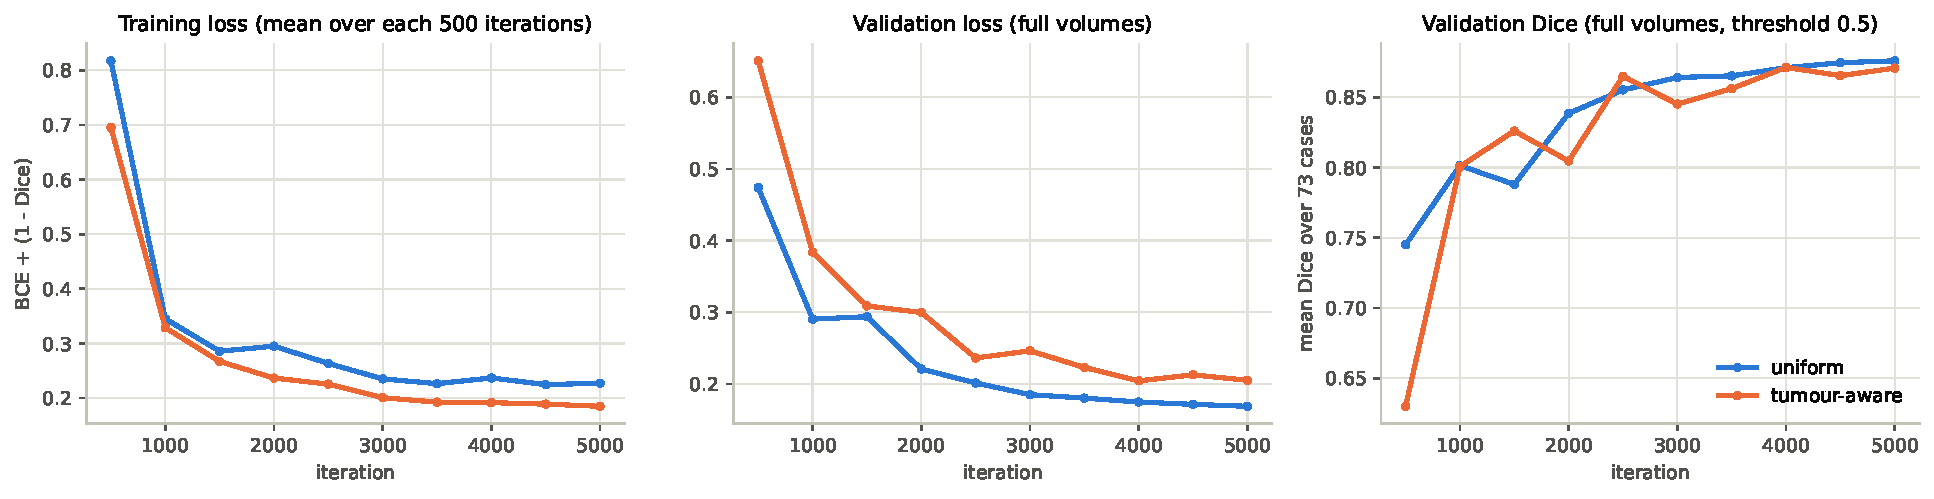
\includegraphics[width=\textwidth]{figures/fig_curves.pdf}
\caption{Learning curves. Training loss is averaged over each 500 iterations; validation metrics use all 73 validation volumes.}
\label{fig:curves}
\end{figure}

\textbf{Curves.} No overfitting: validation loss falls over both runs with small bumps (uniform 0.474$\to$0.169, tumour-aware 0.651$\to$0.205) and validation Dice levels off near 0.87 from about 3{,}500 iterations. Training is budget-limited (mild underfitting): validation loss is still decreasing at the end, and the last 500 iterations add only $+0.001$ Dice because the learning rate has decayed to zero. The tumour-aware run is less stable (Dice drops at 2{,}000 and 3{,}000). Its \emph{lower} training loss with \emph{higher} validation loss reflects its more tumour-rich patch distribution; training losses are not comparable across samplers. No test data were used.

\section{Controlled sampling comparison}
\begin{table}[H]
\centering\small
\caption{Validation (73 cases), final weights, 50\% overlap, threshold 0.5. Paired Wilcoxon signed-rank tests across cases.}
\label{tab:val}
\begin{tabular}{@{}lrrrrrr@{}}\toprule
 & \multicolumn{2}{c}{Uniform} & \multicolumn{2}{c}{Tumour-aware} & \multicolumn{2}{c}{Tumour-aware $-$ uniform} \\
\cmidrule(lr){2-3}\cmidrule(lr){4-5}\cmidrule(l){6-7}
Metric & Mean & Median & Mean & Median & Mean diff. & $p$ \\\midrule
Dice & 0.876 & 0.900 & 0.871 & 0.892 & $-0.005$ & 0.74 \\
Sensitivity & 0.886 & 0.910 & 0.915 & 0.938 & $+0.029$ & $<0.001$ \\
False-positive volume (mL) & 10.8 & 7.6 & 15.5 & 9.9 & $+4.8$ & $<0.001$ \\
False-negative volume (mL) & 10.9 & 7.6 & 7.5 & 5.5 & $-3.3$ & $<0.001$ \\
HD95 (mm) & 16.1 & 6.7 & 25.6 & 8.5 & $+9.5$ & 0.007 \\\bottomrule
\end{tabular}
\end{table}

\textbf{Mechanism.} Dice did not change, but the errors moved (Table~\ref{tab:val}): tumour-aware sampling raised sensitivity in 60 of 73 cases and false-positive volume in 53. Doubling the tumour share of the training voxels shifts the class prior the network learns, pushing its estimate of $P(\text{tumour}\mid\text{appearance})$ upwards. At the fixed 0.5 threshold, borderline voxels flip to tumour: faint outer edema (recovering misses) but also FLAIR-bright non-tumour tissue (new false positives, some far from the tumour, hence the higher HD95). Dice weighs both, so they roughly cancel. The effect is bounded by the data: tumours are large (median $\approx$90\mL, a $\approx$55\mm{} sphere) relative to a 64\mm{} patch, so uniform patches already contain tumour 79\% of the time. With one run per condition, seed-to-seed variability is not estimated.

\textbf{Selection (validation only).} Rule fixed beforehand: higher mean validation Dice, with median HD95 as tie-break within 0.005. \textbf{Uniform} wins (0.8759 vs 0.8707), and the tie-break (6.7 vs 8.5\mm), false-positive volume and validation loss agree, so the choice does not hinge on the margin. \textbf{Disadvantage of excessive oversampling:} the network sees too little healthy tissue, its probabilities become biased towards tumour and it labels tumour-like normal structures as tumour; even $p=0.5$ raised mean false-positive volume by 44\%.

\textbf{Postprocessing rule (validation only).} Remove 26-connected predicted components smaller than $T$\mL. Whole tumour is usually one contiguous region, so small isolated islands are more often false positives, and a size threshold (unlike keep-largest) preserves separate genuine lesions. $T$ was chosen from $\{0.05,0.1,0.25,0.5,1,2\}$\mL{} as the lowest median validation HD95 without lowering mean Dice: \textbf{$T=0.5$\mL} (median HD95 $6.7\to5.8$\mm, Dice $0.876\to0.877$).

\section{Full-volume reconstruction and test evaluation}\label{sec:test}
\textbf{Sliding window.} 64$^3$ windows, 50\% overlap (stride 32; the last window per axis is shifted back to the volume edge), median 80 windows per case. Each window's sigmoid probabilities are multiplied by a 3D Gaussian ($\sigma=8$ voxels, peak at the window centre, as in nnU-Net~\cite{isensee2021}), accumulated and divided by the summed weights, so overlapping \emph{probabilities} are combined before thresholding at 0.5; the mask is pasted back into the original grid. Inference takes 1.0\,s per case.

\begin{table}[H]
\centering\small
\caption{Test split, 73 cases: uniform 64$^3$ model of Section~5 (first evaluation) and v2 pipeline of \hyperref[sec:v2]{Appendix~C} (fixed on validation, evaluated once afterwards). Mean $\pm$ SD (median). HD95: larger of the two directed 95th-percentile distances, mm. No prediction was empty.}
\label{tab:test}
\begin{tabular}{@{}lccc@{}}\toprule
Metric & Before postprocessing & After ($<0.5$\mL{} removed) & v2: tumour96 + flip \\\midrule
Dice & $0.888\pm0.065$ (0.901) & $\mathbf{0.889\pm0.065}$ (0.901) & $\mathbf{0.911\pm0.055}$ (0.927) \\
IoU & $0.805\pm0.099$ (0.819) & $0.806\pm0.098$ (0.820) & $0.840\pm0.086$ (0.865) \\
Sensitivity & $0.888\pm0.086$ (0.906) & $0.887\pm0.086$ (0.906) & $0.912\pm0.061$ (0.928) \\
HD95 (mm) & $9.36\pm11.30$ (5.39) & $9.41\pm10.73$ (5.39) & $7.99\pm11.24$ (4.12) \\
False-positive volume (mL) & $9.93\pm11.69$ (6.92) & $9.78\pm11.63$ (6.92) & $7.67\pm8.28$ (5.43) \\
Absolute volume error (mL) & $11.30\pm12.05$ (6.83) & $11.28\pm12.05$ (6.63) & $7.98\pm7.92$ (5.42) \\
Signed volume error (\%) & $-0.0\pm15.6$ ($-1.1$) & $-0.3\pm15.5$ ($-2.2$) & $+0.6\pm13.0$ ($-1.9$) \\\bottomrule
\end{tabular}
\end{table}

\textbf{Volume.} Volume = voxel count $\times$ ($s_x s_y s_z$)/1000\mL{}, with $s=1$\mm. The median absolute volume error is 6.6\mL{} (8.7\%), with no systematic bias (mean signed error $-0.3$\%); the largest over-estimates ($+45$\%, $+45$\%, $+38$\%) and under-estimates ($-29$\%) are listed in the appendix (Table~\ref{tab:cases}, Fig.~\ref{fig:volumes}).

\textbf{Postprocessing before/after.} The rule fixed on validation is close to neutral on test: Dice $+0.001$, false-positive volume $-0.15$\mL, median HD95 unchanged, mean HD95 slightly \emph{worse}. HD95 improved in 21 cases and worsened in 12; in BRATS\_253 it rose from 10.4 to 32.0\mm{} because 46 of the 77 removed voxels were real, small, separate pieces of tumour, which became distant misses. The rule is kept as fixed, not retuned on test.

\textbf{Effect of near-duplicates.} Test cases with a twin in train or validation score higher (Dice 0.909 vs 0.876, Mann--Whitney $p=0.025$), but not because the model saw the scan: twins in validation or test, never trained on, score as high (0.906, 0.921; $n=6$ each) as training twins (0.910, $n=23$; no twin: 0.869), and predictions are no closer to the twin's training label than to their own (0.915 vs 0.910, closer in 11 of 23, $p=0.92$). This is case mix, so the 73-case result stands; the cost is fewer independent scans (70 in the test split).

\section{Three-plane error analysis}
\begin{figure}[t]
\centering
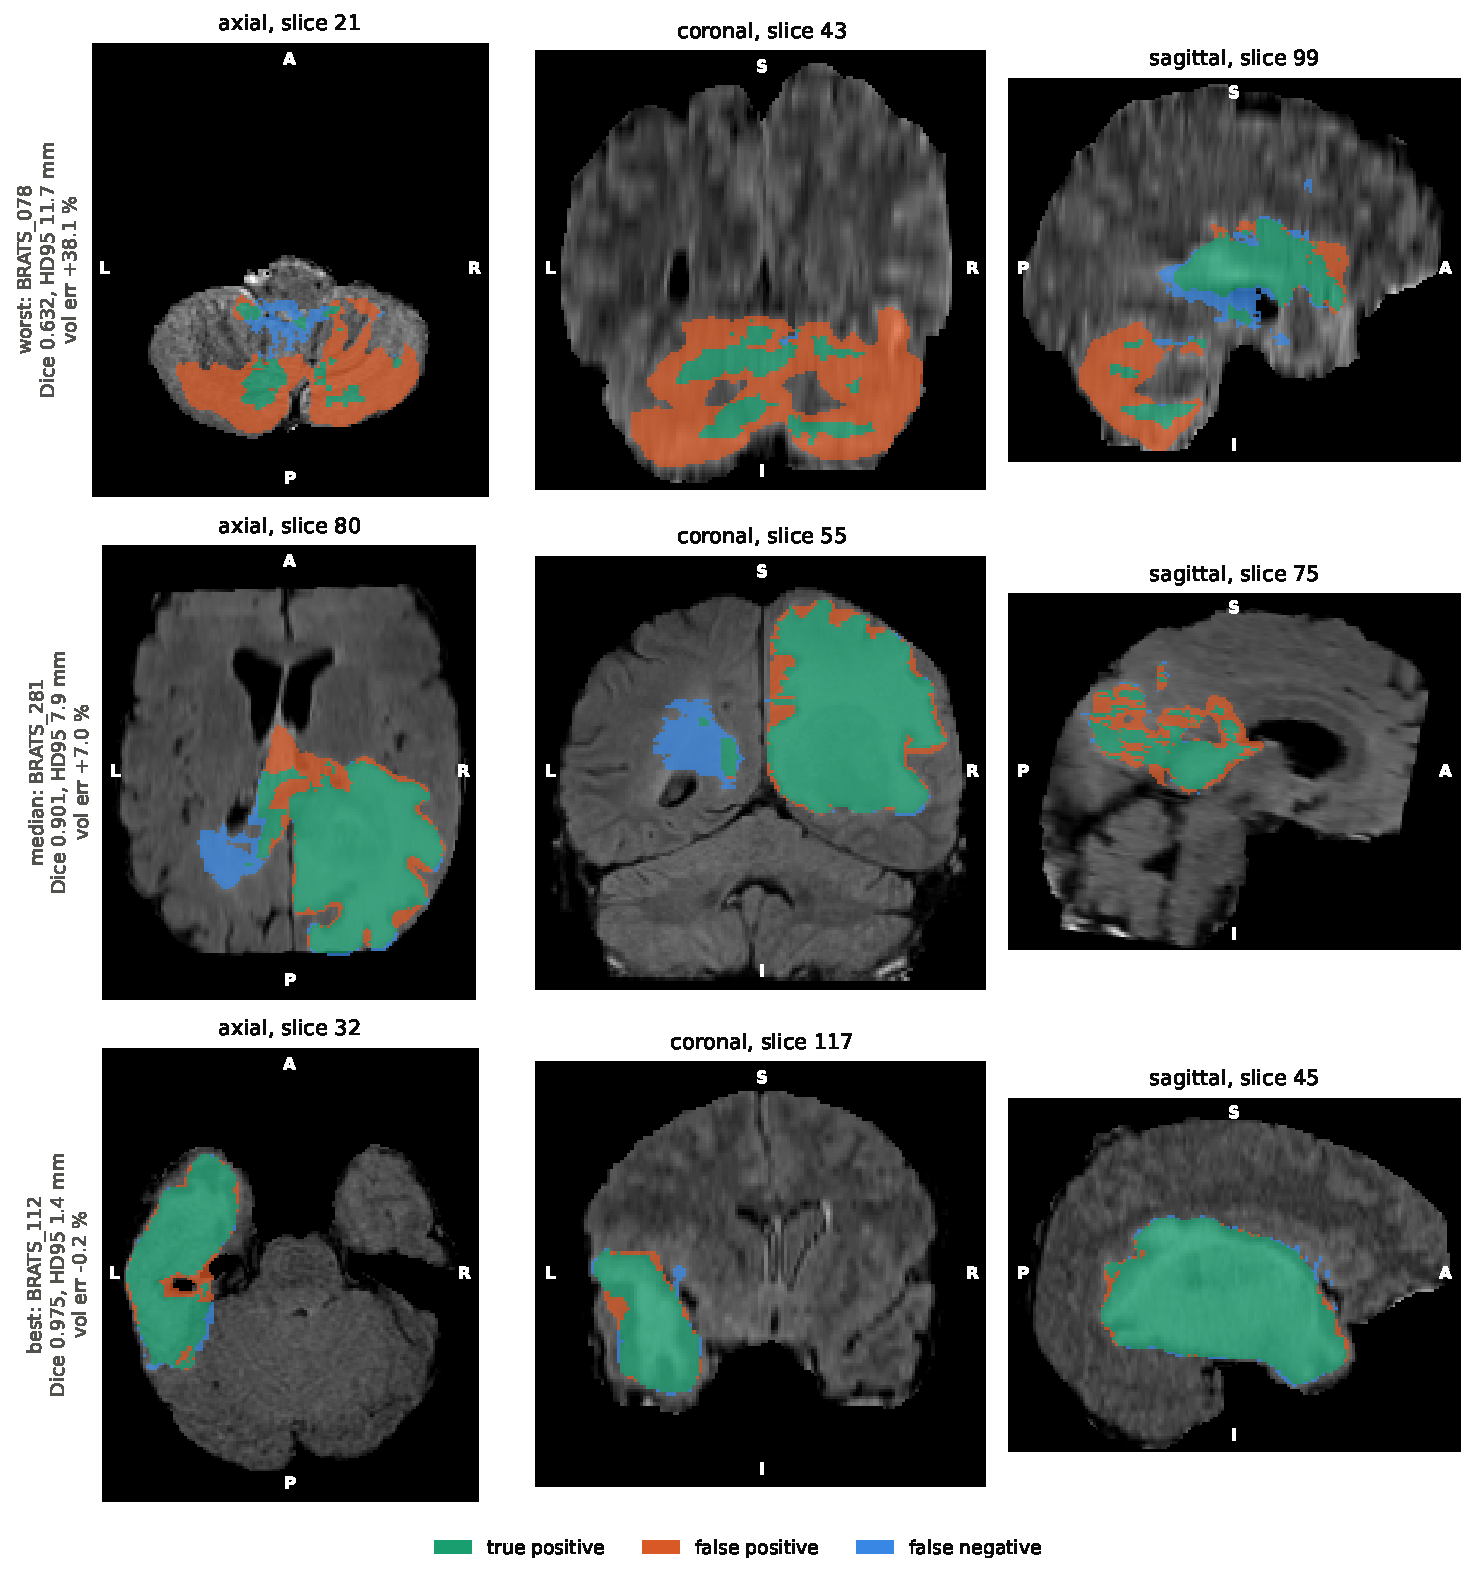
\includegraphics[width=0.63\textwidth]{figures/fig_errors.pdf}
\caption{Worst, median and best test cases by Dice (64$^3$ pipeline of Section~\ref{sec:test}). Each plane is shown at the slice with the most misclassified voxels. Reference = TP + FN, prediction = TP + FP.}
\label{fig:errors}
\end{figure}

\textbf{Errors related to their causes.}
\textbf{Best, BRATS\_112} (Dice 0.975, HD95 1.4\mm): \emph{boundary quality}. Errors form a one-voxel shell; 95\% of missed voxels lie within 2\mm{} of the reference boundary, and FP and FN volumes balance (4.1 vs 4.4\mL). The residual is boundary placement at the 1\mm{} voxel scale, where annotations also disagree.
\textbf{Median, BRATS\_281} (Dice 0.901, HD95 7.9\mm): \emph{a small separate structure}. The main mass is captured, but a separate 8.1\mL{} region of edema in the other hemisphere is entirely missed. It is much less conspicuous (median FLAIR z-score 0.97 vs 1.95 in detected tumour; T2w 0.01 vs 1.48), and the probability there peaks at 0.499, just below the threshold. Its training twin carries an essentially identical label, so this is a weak-signal failure, not unseen anatomy.
\textbf{Worst, BRATS\_078} (Dice 0.632, HD95 11.7\mm, volume +38\%): \emph{over-segmentation of tumour-like tissue}. 53.5\mL{} of false positive lies in the posterior fossa about 30\mm{} below the reference, in moderately FLAIR-bright cerebellar tissue (z 0.95 vs $-0.14$ elsewhere). It is connected to the true tumour (one 118\mL{} component), so the component rule cannot remove it. Limited \emph{patch context} was suspected, but the v2 model with 96\mm{} windows keeps a 50\mL{} false positive there (\hyperref[sec:v2]{Appendix~C}): the tissue itself looks like edema to the model.

\textbf{Dice vs HD95 vs volume error.} Over the test set Dice and HD95 correlate at Spearman $-0.76$, but rankings disagree (Appendix, Fig.~\ref{fig:dicehd}):
\begin{itemize}
\item BRATS\_078 has the lowest Dice but only an 11.7\mm{} HD95, because its false positive is \emph{attached} to the tumour; its volume error (+38\%) is among the largest.
\item BRATS\_481 has near-median Dice (0.89) but the second-highest HD95 (44\mm): one small distant error dominates the 95th percentile.
\item BRATS\_376 has Dice 0.73 but a volume error of only $-6$\%, because 2.4\mL{} of FP and 3.0\mL{} of FN cancel.
\item Tumours $<40$\mL{} average Dice 0.846 against 0.897 for larger ones: the same one-voxel boundary error costs more on a small object.
\end{itemize}
Dice measures size-normalised overlap, HD95 the worst part of the boundary in mm, and volume error the clinically tracked quantity but not \emph{where} errors are. Each misses failures the others catch.\enlargethispage{\baselineskip}

\section{Limitations}
\begin{enumerate}
\item \textbf{Small training budget:} one run per sampler, 5{,}000 iterations of 4 patches (about 75 min each), no hyperparameter search, validation loss still falling (a longer budget helped: \hyperref[sec:v2]{Appendix~C}). Without repeated seeds, a Dice difference of 0.005 could reverse. The shifts in sensitivity, FP volume and HD95 were large and consistent across cases.
\item \textbf{No external-site validation:} all cases come from one curated collection (BraTS via MSD), co-registered, skull-stripped and resampled by one pipeline. Performance on other hospitals, scanners, protocols or preprocessing (or with a missing sequence, Bonus A) is unknown and likely lower.
\item \textbf{Case-level, not scan-level, split:} 29 of 73 test cases have a twin scan in train or validation, 26 of 73 validation cases one in training. Twin cases score higher through case mix, not measurable memorisation (Section~\ref{sec:test}), but only 368 scans are independent, and the longer-trained v2 leans slightly towards training labels ($p=0.10$).
\item \textbf{Uncertain reference:} research annotations, not pathology; two annotations of the same scan agree at Dice 0.92 on average, which bounds what any score against one of them means.
\item \textbf{Fixed, uncalibrated choices:} threshold 0.5, 64$^3$ patch and 50\% overlap were fixed a priori. Probabilities are not calibrated (the sampler visibly shifts them). Only whole tumour was modelled. Laterality comes from the header alone.
\end{enumerate}

\section{Bonus A: missing-modality stress test}
\begin{wrapfigure}[8]{r}{0.42\textwidth}
\vspace{-12pt}
\centering
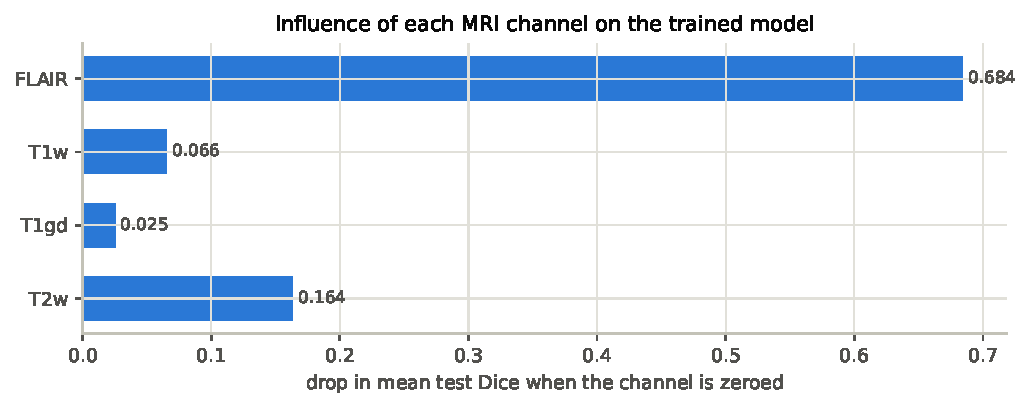
\includegraphics[width=0.42\textwidth]{figures/fig_bonus_modality.pdf}
\vspace{-14pt}
\end{wrapfigure}
Each channel was set to zero at test time without retraining (64$^3$ pipeline of Section~\ref{sec:test}, 73 test cases). Mean Dice: all four channels 0.889; FLAIR zeroed \textbf{0.205} (29 empty predictions, median volume error $-97$\%); T2w zeroed 0.726 (median $-22$\%); T1w zeroed 0.824 (median $+22$\%, median HD95 $5.4\to31.9$\mm); T1gd zeroed 0.864.

\textbf{FLAIR is the most influential channel}, then T2w. This matches the target: whole tumour is dominated by edema, which is defined by FLAIR/T2 hyperintensity, whereas T1gd mainly outlines the enhancing core, a small part of the volume. Zeroing is an imperfect simulation of a missing acquisition. After brain z-scoring, 0 is not ``no information'' but the channel's mean brain intensity, so the network sees a flat average-tissue image it never met in training and cannot recognise as missing. Its response is out-of-distribution behaviour (over-segmentation without T1w, under-segmentation without FLAIR/T2w), not graceful degradation. A real missing sequence would also be known in advance, which this model cannot be told. Training could be redesigned with \emph{modality dropout}: randomly drop channels per patch and add a per-channel availability indicator, so the network learns every subset and knows which one it has. Alternatives are per-modality encoders fused by order-invariant pooling (HeMIS~\cite{havaei2016}) or separate models for common sequence subsets.

\section{Bonus B: sliding-window seam test}
\begin{figure}[t]
\centering
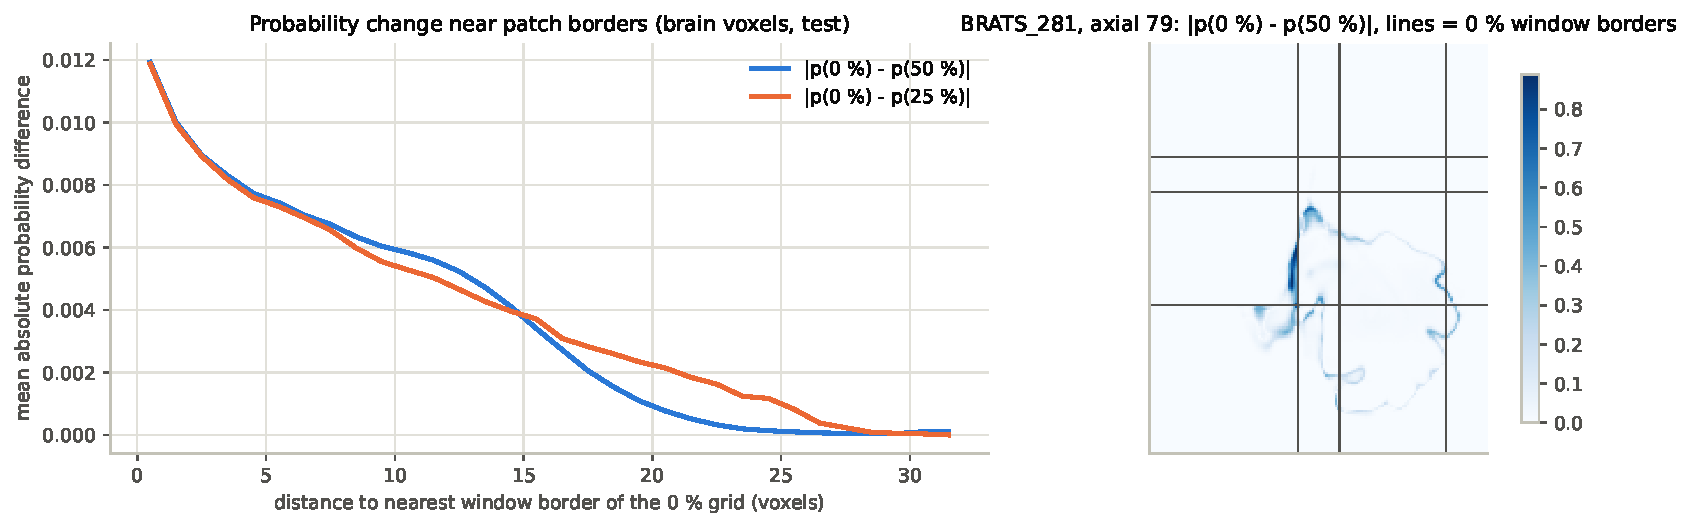
\includegraphics[width=0.78\textwidth]{figures/fig_bonus_seam.pdf}
\caption{Left: mean $|p_{0\%}-p_{50\%}|$ and $|p_{0\%}-p_{25\%}|$ over test brain voxels versus distance to the nearest 0\%-grid window border. Right: difference map for BRATS\_281 with the 0\% window borders.}
\label{fig:seam}
\end{figure}
\begin{table}[H]
\centering\small
\begin{tabular}{@{}lrrrrrrr@{}}\toprule
Overlap & Stride & Windows & s/case & Mean Dice & Median Dice & Median HD95 & Mean HD95 \\\midrule
0\% & 64 & 27 & 0.35 & 0.872 & 0.897 & 5.1 & 10.1 \\
25\% & 48 & 36 & 0.45 & 0.884 & 0.900 & 5.4 & 9.1 \\
50\% & 32 & 80 & 0.99 & 0.889 & 0.901 & 5.4 & 9.4 \\\bottomrule
\end{tabular}
\end{table}
Runtime scales with the number of windows (50\% is $2.8\times$ slower than 0\%). Accuracy improves less: mean Dice $+0.017$, median Dice almost unchanged, median HD95 not better. The gain comes from a minority of cases with poor predictions near window borders. Fig.~\ref{fig:seam} shows the mechanism: the 0\% vs 50\% difference is largest exactly at window borders ($\approx$0.012) and fades to almost nothing 25--30 voxels inside. Border voxels are predicted with one-sided context and zero padding, so overlap (with Gaussian weighting) lets each be predicted again from a window where it is central. Overlap helps most when structures are large relative to the window and cross its borders, as here, and least when the window is large or the object sits inside one window. (At ``0\%'' the last window per axis still overlaps its neighbour.) Choosing the overlap by repeatedly comparing these test results would turn the test set into a tuning set: the setting that happens to fit these 73 cases best would be chosen, and its score would be biased upwards. The 50\% overlap was fixed before the test split was evaluated; this test only describes the effect.

\begin{thebibliography}{9}\footnotesize
\setlength{\itemsep}{0pt}
\bibitem{antonelli2022} M.~Antonelli, A.~Reinke, S.~Bakas, et al. The Medical Segmentation Decathlon. \emph{Nature Communications}, 13:4128, 2022. doi:10.1038/s41467-022-30695-9.
\bibitem{msd2018} Medical Segmentation Decathlon Organizers. Medical Segmentation Decathlon: Task01 BrainTumour. \url{http://medicaldecathlon.com/}, 2018. Data obtained from the MONAI mirror named in the brief, November 2026. Licence CC-BY-SA 4.0.
\bibitem{menze2015} B.~H. Menze, A.~Jakab, S.~Bauer, et al. The multimodal brain tumor image segmentation benchmark (BRATS). \emph{IEEE Trans. Medical Imaging}, 34(10):1993--2024, 2015. doi:10.1109/TMI.2014.2377694.
\bibitem{ronneberger2015} O.~Ronneberger, P.~Fischer, T.~Brox. U-Net: convolutional networks for biomedical image segmentation. \emph{MICCAI}, LNCS 9351, 234--241, 2015.
\bibitem{cicek2016} \"O.~\c{C}i\c{c}ek, A.~Abdulkadir, S.~S. Lienkamp, T.~Brox, O.~Ronneberger. 3D U-Net: learning dense volumetric segmentation from sparse annotation. \emph{MICCAI}, LNCS 9901, 424--432, 2016.
\bibitem{isensee2021} F.~Isensee, P.~F. Jaeger, S.~A.~A. Kohl, J.~Petersen, K.~H. Maier-Hein. nnU-Net: a self-configuring method for deep learning-based biomedical image segmentation. \emph{Nature Methods}, 18:203--211, 2021.
\bibitem{havaei2016} M.~Havaei, N.~Guizard, N.~Chapados, Y.~Bengio. HeMIS: hetero-modal image segmentation. \emph{MICCAI}, LNCS 9901, 469--477, 2016.
\end{thebibliography}

\clearpage
\appendix
\section*{Appendix A. Per-case test results (64$^3$ pipeline of Section~\ref{sec:test})}
\begin{table}[H]
\centering
\caption{All 73 test cases, uniform model with the 0.5\mL{} component rule. $^\dagger$ = scan also present (as a twin) in train or validation. $\Delta V$ = signed volume error.}
\label{tab:cases}
{\scriptsize\setlength{\tabcolsep}{3pt}
\begin{tabular}{@{}lrrrrrrrr@{}}\toprule
Case & Dice & IoU & Sens. & HD95 & Ref & Pred & $|\Delta V|$ & $\Delta V$ \\
 & & & & mm & mL & mL & mL & \% \\\midrule
002 & 0.888 & 0.799 & 0.989 & 4.0 & 63.1 & 77.3 & 14.3 & +22.6 \\
012$^\dagger$ & 0.908 & 0.832 & 0.910 & 8.1 & 21.6 & 21.7 & 0.1 & +0.4 \\
016$^\dagger$ & 0.891 & 0.804 & 0.966 & 4.2 & 82.7 & 96.6 & 13.9 & +16.8 \\
033$^\dagger$ & 0.951 & 0.907 & 0.968 & 2.0 & 114.0 & 118.0 & 4.0 & +3.5 \\
039 & 0.836 & 0.719 & 0.729 & 7.0 & 37.0 & 27.5 & 9.5 & -25.6 \\
050$^\dagger$ & 0.924 & 0.860 & 0.891 & 4.1 & 76.2 & 70.8 & 5.5 & -7.2 \\
059 & 0.936 & 0.879 & 0.905 & 3.3 & 99.6 & 93.1 & 6.5 & -6.5 \\
065$^\dagger$ & 0.855 & 0.747 & 0.880 & 6.7 & 166.1 & 175.8 & 9.8 & +5.9 \\
067 & 0.944 & 0.894 & 0.911 & 2.2 & 55.3 & 51.4 & 3.9 & -7.0 \\
078 & 0.632 & 0.462 & 0.752 & 11.7 & 85.1 & 117.5 & 32.4 & +38.1 \\
079$^\dagger$ & 0.924 & 0.859 & 0.902 & 2.2 & 89.1 & 84.9 & 4.3 & -4.8 \\
088 & 0.925 & 0.861 & 0.902 & 4.6 & 253.7 & 240.9 & 12.8 & -5.0 \\
097 & 0.957 & 0.917 & 0.974 & 2.0 & 153.2 & 158.8 & 5.6 & +3.7 \\
108 & 0.866 & 0.763 & 0.883 & 8.3 & 121.8 & 126.6 & 4.8 & +3.9 \\
112 & 0.975 & 0.951 & 0.974 & 1.4 & 169.2 & 168.8 & 0.4 & -0.2 \\
131$^\dagger$ & 0.836 & 0.719 & 0.775 & 11.6 & 173.3 & 148.1 & 25.2 & -14.6 \\
137$^\dagger$ & 0.922 & 0.855 & 0.872 & 6.5 & 147.0 & 131.4 & 15.7 & -10.7 \\
141 & 0.896 & 0.812 & 0.853 & 9.5 & 268.7 & 242.7 & 26.0 & -9.7 \\
142$^\dagger$ & 0.961 & 0.924 & 0.960 & 2.2 & 166.2 & 166.0 & 0.1 & -0.1 \\
144 & 0.934 & 0.876 & 0.898 & 9.2 & 51.3 & 47.3 & 4.0 & -7.8 \\
156 & 0.918 & 0.849 & 0.896 & 3.2 & 222.6 & 212.0 & 10.6 & -4.8 \\
158 & 0.928 & 0.866 & 0.868 & 3.0 & 49.2 & 42.9 & 6.4 & -12.9 \\
163 & 0.891 & 0.804 & 0.820 & 10.0 & 78.4 & 65.8 & 12.5 & -16.0 \\
168$^\dagger$ & 0.817 & 0.691 & 0.837 & 10.3 & 40.5 & 42.4 & 1.9 & +4.8 \\
169 & 0.816 & 0.689 & 0.726 & 13.9 & 87.4 & 68.2 & 19.2 & -22.0 \\
171 & 0.933 & 0.874 & 0.952 & 2.0 & 20.6 & 21.4 & 0.9 & +4.1 \\
173$^\dagger$ & 0.962 & 0.927 & 0.964 & 1.4 & 179.3 & 180.1 & 0.8 & +0.5 \\
188 & 0.781 & 0.640 & 0.820 & 14.0 & 35.8 & 39.5 & 3.6 & +10.2 \\
192 & 0.841 & 0.725 & 0.796 & 6.1 & 96.8 & 86.5 & 10.3 & -10.7 \\
198 & 0.952 & 0.909 & 0.925 & 6.1 & 181.0 & 170.5 & 10.5 & -5.8 \\
222$^\dagger$ & 0.929 & 0.868 & 0.919 & 15.8 & 78.3 & 76.6 & 1.7 & -2.2 \\
230 & 0.854 & 0.744 & 0.822 & 3.6 & 28.3 & 26.2 & 2.1 & -7.4 \\
241 & 0.797 & 0.662 & 0.977 & 16.2 & 134.6 & 195.5 & 60.9 & +45.3 \\
246 & 0.823 & 0.699 & 0.702 & 36.2 & 81.4 & 57.5 & 23.9 & -29.4 \\
247 & 0.862 & 0.758 & 0.762 & 29.5 & 74.0 & 56.9 & 17.1 & -23.1 \\
249 & 0.937 & 0.881 & 0.921 & 9.2 & 318.3 & 307.5 & 10.9 & -3.4 \\
250 & 0.902 & 0.822 & 0.927 & 12.6 & 166.6 & 175.6 & 9.0 & +5.4 \\
\bottomrule
\end{tabular}
\hfill
\begin{tabular}{@{}lrrrrrrrr@{}}\toprule
Case & Dice & IoU & Sens. & HD95 & Ref & Pred & $|\Delta V|$ & $\Delta V$ \\
 & & & & mm & mL & mL & mL & \% \\\midrule
252$^\dagger$ & 0.926 & 0.862 & 0.903 & 3.5 & 79.9 & 75.9 & 3.9 & -4.9 \\
253 & 0.897 & 0.814 & 0.854 & 32.0 & 54.4 & 49.1 & 5.2 & -9.6 \\
260 & 0.957 & 0.918 & 0.942 & 2.2 & 108.4 & 104.9 & 3.5 & -3.2 \\
262 & 0.896 & 0.812 & 0.860 & 3.2 & 23.9 & 22.0 & 2.0 & -8.1 \\
281$^\dagger$ & 0.901 & 0.820 & 0.933 & 7.9 & 173.9 & 186.2 & 12.3 & +7.0 \\
283$^\dagger$ & 0.933 & 0.874 & 0.944 & 3.3 & 217.4 & 222.3 & 5.0 & +2.3 \\
293 & 0.888 & 0.799 & 0.989 & 4.0 & 63.1 & 77.3 & 14.3 & +22.6 \\
303 & 0.884 & 0.793 & 0.833 & 5.4 & 183.1 & 161.9 & 21.2 & -11.6 \\
305 & 0.895 & 0.810 & 0.968 & 11.2 & 55.1 & 64.1 & 9.0 & +16.3 \\
307 & 0.869 & 0.768 & 0.910 & 42.3 & 46.3 & 50.7 & 4.4 & +9.5 \\
322 & 0.866 & 0.763 & 0.935 & 4.1 & 20.9 & 24.3 & 3.4 & +16.0 \\
341 & 0.885 & 0.794 & 0.832 & 11.1 & 132.7 & 116.7 & 16.0 & -12.0 \\
354 & 0.928 & 0.865 & 0.939 & 6.4 & 87.3 & 89.5 & 2.2 & +2.5 \\
366 & 0.734 & 0.580 & 0.899 & 11.4 & 89.2 & 129.1 & 39.9 & +44.7 \\
372 & 0.797 & 0.662 & 0.858 & 38.8 & 39.4 & 45.5 & 6.1 & +15.5 \\
374 & 0.864 & 0.760 & 0.942 & 5.4 & 43.5 & 51.4 & 7.9 & +18.2 \\
376 & 0.729 & 0.574 & 0.707 & 25.0 & 10.1 & 9.5 & 0.6 & -6.0 \\
377 & 0.897 & 0.813 & 0.986 & 3.0 & 73.7 & 88.3 & 14.7 & +19.9 \\
387$^\dagger$ & 0.937 & 0.881 & 0.937 & 4.1 & 150.8 & 150.9 & 0.1 & +0.0 \\
396$^\dagger$ & 0.943 & 0.892 & 0.907 & 1.7 & 110.2 & 101.6 & 8.5 & -7.7 \\
399$^\dagger$ & 0.946 & 0.897 & 0.993 & 2.2 & 163.6 & 180.0 & 16.4 & +10.0 \\
401 & 0.925 & 0.860 & 0.993 & 2.8 & 44.8 & 51.4 & 6.6 & +14.8 \\
412$^\dagger$ & 0.922 & 0.855 & 0.875 & 4.6 & 172.7 & 155.1 & 17.5 & -10.2 \\
414$^\dagger$ & 0.820 & 0.695 & 0.703 & 13.4 & 156.8 & 112.1 & 44.6 & -28.5 \\
436 & 0.955 & 0.914 & 0.944 & 2.4 & 43.9 & 42.9 & 1.0 & -2.3 \\
437$^\dagger$ & 0.901 & 0.819 & 0.989 & 4.4 & 129.8 & 155.4 & 25.6 & +19.7 \\
440$^\dagger$ & 0.909 & 0.833 & 0.954 & 2.4 & 66.8 & 73.4 & 6.6 & +9.9 \\
447$^\dagger$ & 0.950 & 0.905 & 0.924 & 2.8 & 107.2 & 101.3 & 5.9 & -5.5 \\
451$^\dagger$ & 0.967 & 0.937 & 0.961 & 1.4 & 186.3 & 183.9 & 2.3 & -1.3 \\
453$^\dagger$ & 0.830 & 0.710 & 0.722 & 8.5 & 134.3 & 99.3 & 35.0 & -26.0 \\
461$^\dagger$ & 0.957 & 0.917 & 0.962 & 2.2 & 148.0 & 149.6 & 1.6 & +1.1 \\
462$^\dagger$ & 0.780 & 0.640 & 0.669 & 46.8 & 38.3 & 27.4 & 10.9 & -28.5 \\
466$^\dagger$ & 0.923 & 0.857 & 0.974 & 2.0 & 16.7 & 18.6 & 1.9 & +11.1 \\
467$^\dagger$ & 0.944 & 0.893 & 0.905 & 2.2 & 157.7 & 144.7 & 13.0 & -8.2 \\
481 & 0.885 & 0.794 & 0.924 & 44.3 & 57.2 & 62.1 & 5.0 & +8.7 \\
482 & 0.769 & 0.624 & 0.667 & 13.7 & 184.7 & 136.0 & 48.7 & -26.4 \\
\bottomrule
\end{tabular}
}

\end{table}

\section*{Appendix B. Supporting figures}
\begin{figure}[H]
\centering
\begin{minipage}[t]{0.49\textwidth}\centering
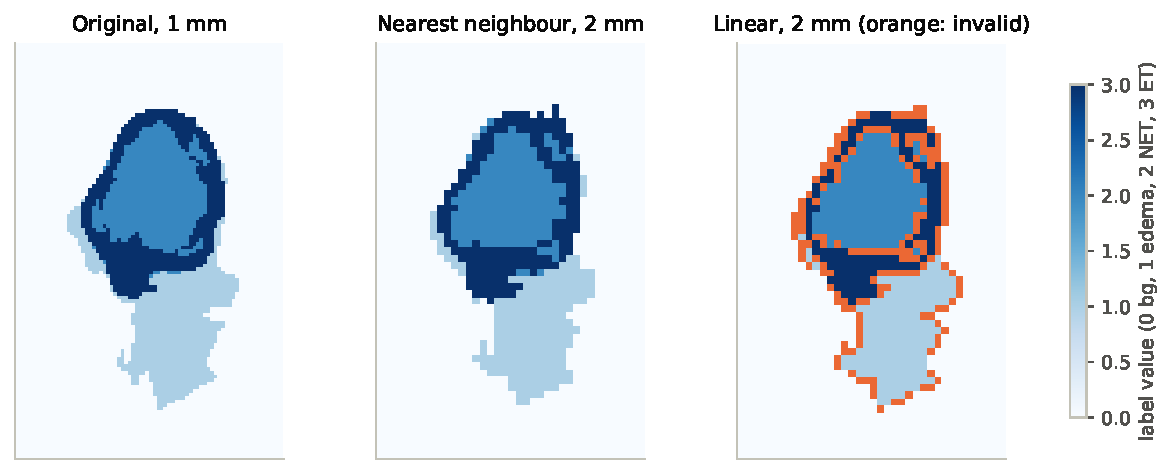
\includegraphics[width=\textwidth]{figures/fig_interpolation.pdf}
\caption{Label resampled to 2\mm{}: nearest neighbour keeps valid classes; linear interpolation creates invalid values (orange).}
\label{fig:interp}
\end{minipage}\hfill
\begin{minipage}[t]{0.47\textwidth}\centering
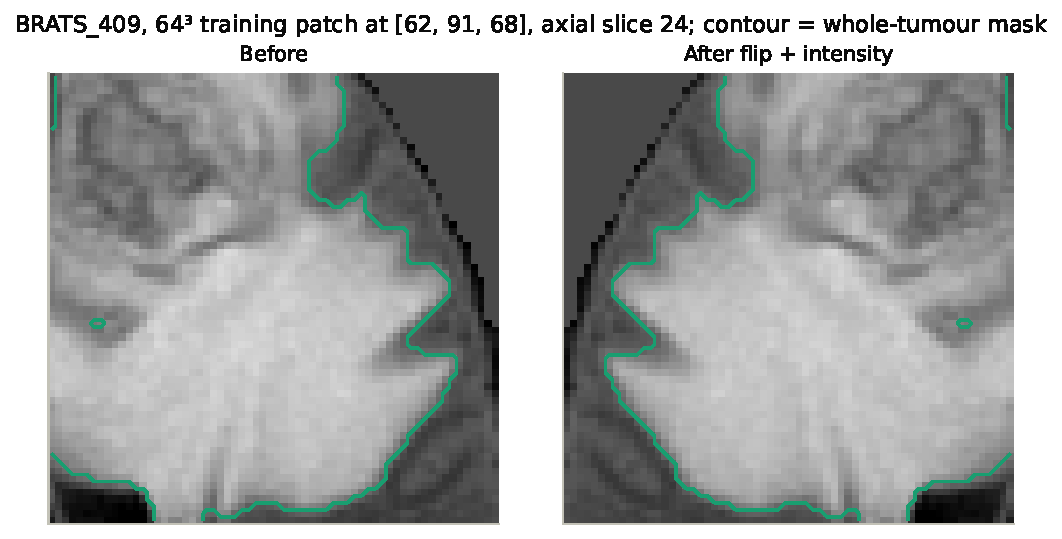
\includegraphics[width=\textwidth]{figures/fig_augmentation.pdf}
\caption{Paired training-only augmentation on a real 64$^3$ patch: left--right flip and intensity change; the mask (contour) follows the image.}
\label{fig:aug}
\end{minipage}
\end{figure}
\begin{figure}[H]
\centering
\begin{minipage}[t]{0.49\textwidth}\centering
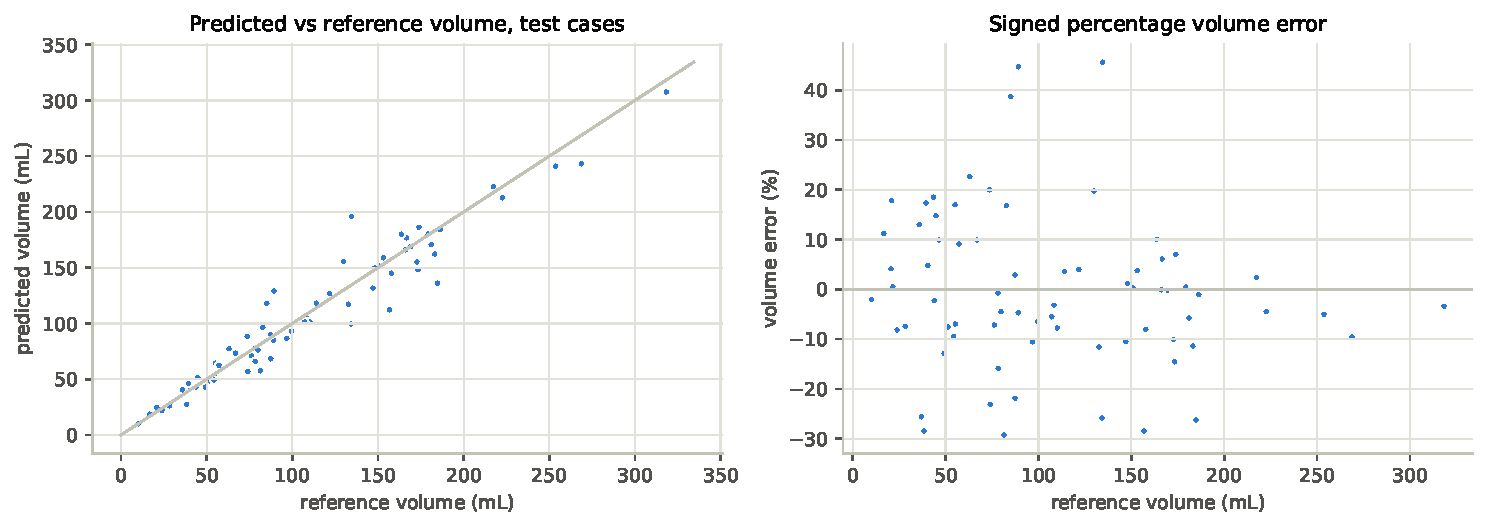
\includegraphics[width=\textwidth]{figures/fig_volumes.pdf}
\caption{Test volumes (before postprocessing): predicted vs reference, and signed percentage error.}
\label{fig:volumes}
\end{minipage}\hfill
\begin{minipage}[t]{0.49\textwidth}\centering
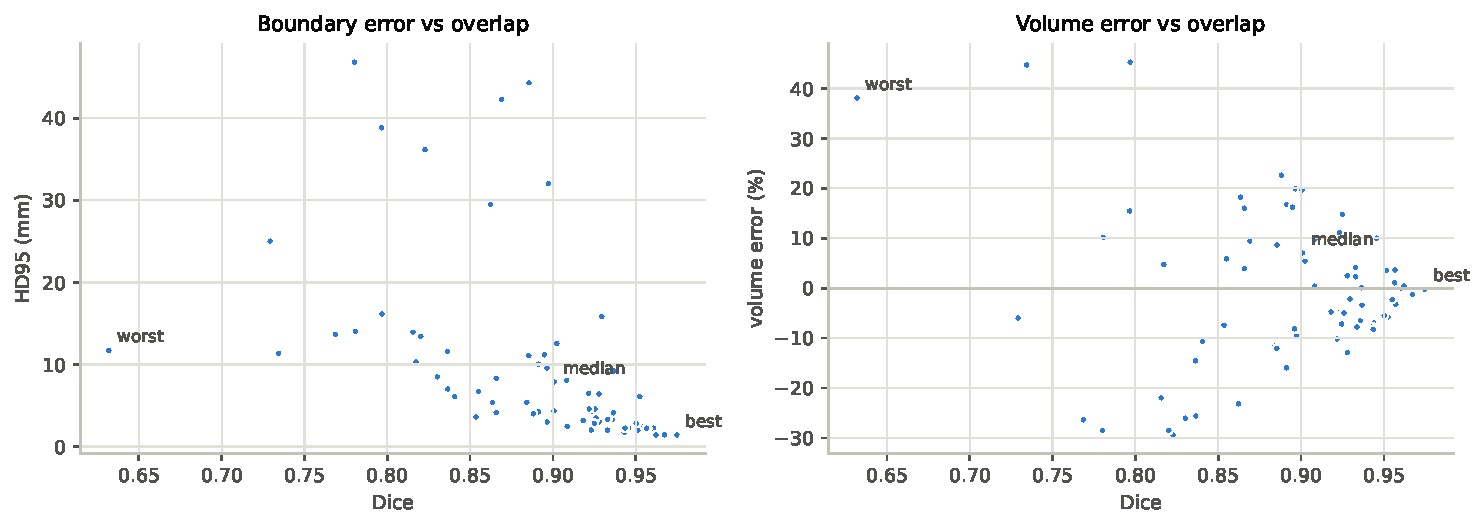
\includegraphics[width=\textwidth]{figures/fig_dice_hd95.pdf}
\caption{Test cases: HD95 and signed volume error against Dice; best, median and worst cases labelled.}
\label{fig:dicehd}
\end{minipage}
\end{figure}
\begin{figure}[H]
\centering
\begin{minipage}[t]{0.49\textwidth}\centering
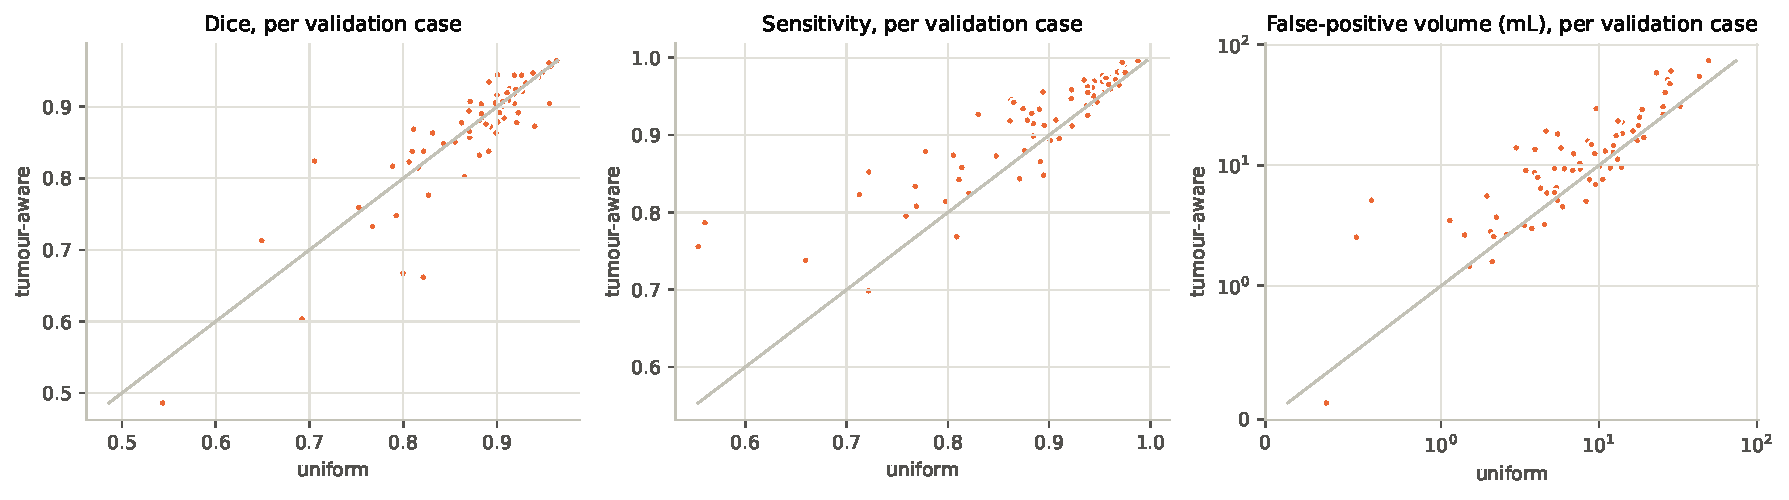
\includegraphics[width=\textwidth]{figures/fig_val_comparison.pdf}
\caption{Validation, per case: tumour-aware against uniform for Dice, sensitivity and false-positive volume.}
\end{minipage}\hfill
\begin{minipage}[t]{0.47\textwidth}\centering
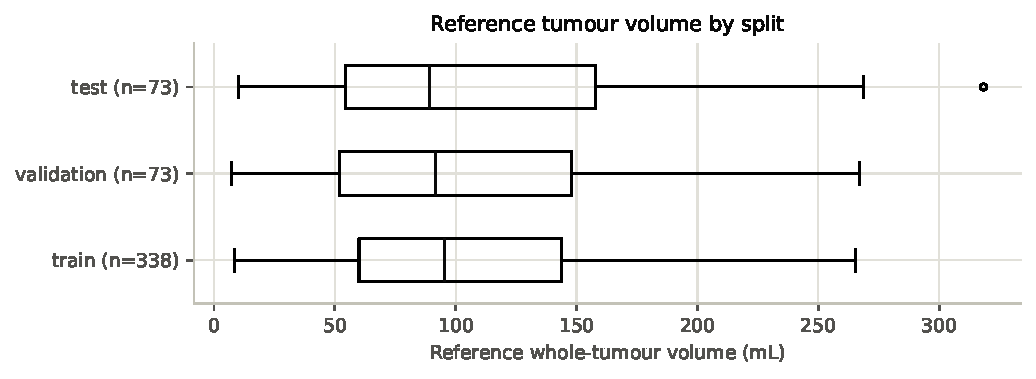
\includegraphics[width=\textwidth]{figures/fig_split_volumes.pdf}
\caption{Reference whole-tumour volume by split.}
\end{minipage}
\end{figure}

\section*{Appendix C. Beyond the brief: improved pipeline (v2)}\phantomsection\label{sec:v2}
\textbf{Training.} After the test evaluation of Section~\ref{sec:test}, both samplers were retrained with \textbf{96$^3$ patches $\times$ 2 for 40{,}000 iterations} (13$\times$ the training voxels) and stronger training-only augmentation: rotation up to $\pm15^\circ$ and scaling $\times0.9$--1.1 ($p=0.25$), per-channel gamma ($p=0.3$) and Gaussian noise ($p=0.15$). Loss, optimiser, schedule, seed and initial weights are unchanged. On Apple's MPS backend the weight gradient of 3D convolutions is slow; computing each $3^3$ convolution as one 2D convolution over three depth-shifted copies of the input (same parameters; logits agree to within $3\times10^{-5}$) made training $3\times$ faster, 4.5\,h per run (notebook Section~10).

\textbf{Selection (validation only; rule fixed in code before any v2 result).} Candidates were either model alone, with left--right flip averaging, or both models averaged, at thresholds 0.4, 0.5 and 0.6; the simplest option within 0.002 mean Dice of the best wins. Each 96$^3$ model alone reaches 0.908--0.909 validation Dice (64$^3$ uniform: 0.876), and flipping and averaging add at most 0.004, so \textbf{tumour96 + flip at threshold 0.5} was selected (0.911; best option 0.913, paired $p=0.17$). No component threshold lowered the median validation HD95, so by the Section~5 criterion v2 has no postprocessing. At 96$^3$ the samplers barely differ in class balance (tumour share of patch voxels 7.0 vs 8.9\%, against 7.2 vs 16.1\% at 64$^3$), and the tumour-aware error shift almost vanishes (sensitivity $+0.005$, FP volume $-0.1$\mL), which supports the mechanism of Section~5.

\textbf{Test, evaluated once with the frozen pipeline} (Table~\ref{tab:test}). Dice $0.889\to\mathbf{0.911}$, better in 62 of 73 cases (Wilcoxon $p<0.001$); median HD95 $5.4\to4.1$\mm; FP volume $9.8\to7.7$\mL; median absolute volume error $6.6\to5.4$\mL; 1.05\,s per case. The gain is largest for cases without any twin ($0.869\to0.894$, $n=38$), so it does not come from memorised scans, although v2's predictions lean slightly towards the twins' training labels (closer in 16 of 23 cases, $p=0.10$; v1: 11 of 23, $p=0.92$). The worst case (BRATS\_078, $0.632\to0.692$) keeps its posterior-fossa false positive. \textbf{Caveats:} the test split had been evaluated once before this work, although no v2 choice used it; patch size, budget and augmentation changed together; one run per condition.

\end{document}
